% Generated by ic_study.analysis.v4_report_export from the v4 report with
% manifest SHA-256 6608b3960eb73011caca97870a4ffd3dbfbcd4c2df09bbbcb576c1c9452cf981.
% Edited during the journal revision (agent S, 2026-10-13): captions, headers and
% categorical cells in plain English; every number keeps its \resultnum binding.
\begin{figure*}[tp]
\centering
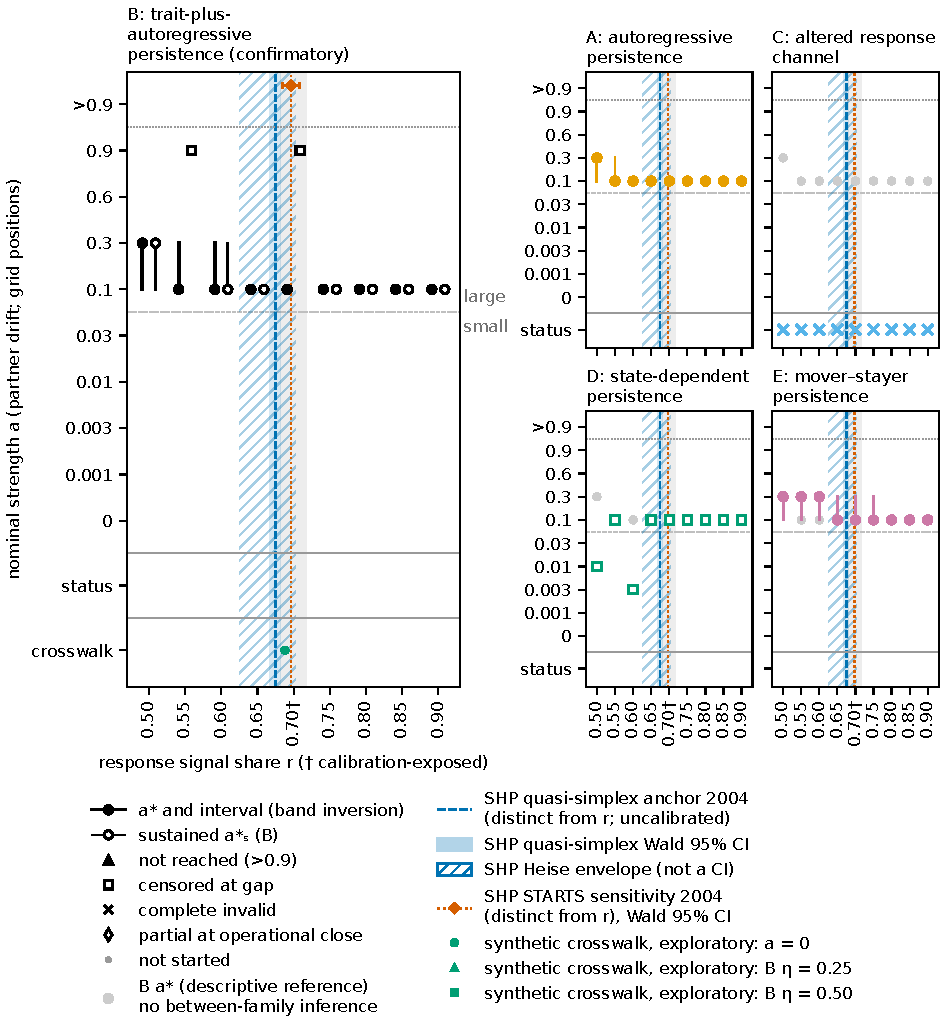
\includegraphics[width=\textwidth,height=175mm,keepaspectratio]{generated/F6_a_star_shp_anchor.pdf}
\caption{Empirical reliability anchor placed on the signal-share axis of the first boundaries $a^*(r)$ against each persistence model (display of the rule-assembled record): the quasi-simplex reliability of the SHP trust item in 2004 (dashed) with its model-based Wald 95\% interval (shaded), the range of the nine three-wave Heise estimates (hatched; a specification range, not a confidence interval), the admissible trait--state--error (STARTS) sensitivity with its Wald interval (dotted), and, in the crosswalk row, the grid value of $r$ whose synthetic crosswalk range contains the SHP estimate ($r=0.70$ for the zero-strength reference; no grid value for either B reference). The empirical reliability and the design signal share are different quantities, the crosswalk ranges are descriptive and do not propagate the uncertainty of the anchor, and nothing is interpolated, extrapolated or rounded to a grid value. Gray B markers in the panels of the other models are a visual reference only. Source: Swiss Household Panel (SHP).}\label{fig:v4-F6}
\end{figure*}
